
\documentclass[10pt]{article}
\linespread{1.25}

%%Make Parenthesis scale to fit whats inside
\newcommand{\parry}[1]{\left( #1 \right)}

%% Language and font encodings
\usepackage[english]{babel}
\usepackage[utf8x]{inputenc}
\usepackage[T1]{fontenc}
\usepackage{subcaption}
\usepackage[section]{placeins}

%% Sets page size and margins
\usepackage[a4paper,top=3cm,bottom=2cm,left=3cm,right=3cm,marginparwidth=1.75cm]{geometry}

%% No indents
\setlength\parindent{0pt}

%% Useful packages
\usepackage{amsmath}
\usepackage{amssymb}
\usepackage{amsfonts}
\usepackage{mathtools}
\usepackage{graphicx}
\usepackage{xcolor}
\usepackage[colorinlistoftodos]{todonotes}
\usepackage[colorlinks=true, allcolors=blue]{hyperref}
\usepackage{enumerate}
\usepackage{enumitem}
\usepackage[framed,autolinebreaks,useliterate]{mcode} %% MATLAB code
\usepackage{siunitx}
\usepackage{float}
\usepackage{scrextend}
\usepackage[final]{pdfpages}

%%Header & Footer
\usepackage[myheadings]{fullpage}
\usepackage{fancyhdr}
\usepackage{lastpage}
\usepackage{graphicx, wrapfig, subcaption, setspace, booktabs}

%% Define \therefore command
\def\therefore{\boldsymbol{\text{ }
\leavevmode
\lower0.4ex\hbox{$\cdot$}
\kern-.5em\raise0.7ex\hbox{$\cdot$}
\kern-0.55em\lower0.4ex\hbox{$\cdot$}
\thinspace\text{ }}}
\renewcommand{\vec}[1]{\boldsymbol{#1}}

%% Units
\DeclareSIUnit\year{yr}
\DeclareSIUnit\dollar{\$}
\DeclareSIUnit\celcius{C^{\circ}}
\DeclareSIUnit\mole{mole}
\def\conclusion{\quad \Rightarrow \quad}

\begin{document}


%----------------------------------------------------------------------------------------
%	TITLE PAGE
%----------------------------------------------------------------------------------------

%----------------------------------------------------------------------------------------
% HEADER AND FOOTER
%----------------------------------------------------------------------------------------
\pagestyle{fancy}
\fancyhf{}
\setlength\headheight{12pt}
\fancyhead[L]{\textbf{ES-APPM 447: Boundary Integral Methods}}
\fancyhead[R]{\textbf{HW 3 \qquad 6/9/2021 \qquad Liam O'Connor}}
\fancyfoot[R]{Page \thepage\ of \pageref{LastPage}}

\textbf{\textit{I used $i$ as both an index as well as the unit imaginary number, in hindsight that was a poor choice.}}

\section*{Problem Statement}
Consider the integro-differential equation
\begin{align}
    \frac{d^2h}{dx^2} + h + \frac{i}{2} \int_{-\pi/2}^{\pi/2} H^1_0 \big( |x - y| \big) h(y)dy &= e^{iax}
\end{align}
for $-\pi/2 \leq x \leq \pi/2$. 
The complex dependent variable $h(x)$ satisfies the boundary conditions $h(\pi/2) = h(-\pi/2) = 0$. 
This equation describes the interface displacement resulting from the scattering of an acoustic wave from an interface separating two fluids.
Here $H^1_0$ is a Hankel function of the first kind.
\begin{enumerate}
    \item Describe a numerical method to solve this differential equation.
    
    \item Solve this equation numerically for $a = 0.1$. 
    Do a numerical convergence check to show convergence of your numerical scheme and use these results to estimate the rate of convergence of your scheme.
    Plot the solution.

    \item Solve the equation for $a = 1.0$.

    \item Explain the differences between the $a = 0.1$ case and the $a = 1.0$ case.
    When can such differences be expected?

\end{enumerate}

\section*{Methods}
\subsection*{General Strategy}
We will solve the equation by discretizing the domain as well as the region of integration uniformly in grid space.
Given a resolution $N$, we define
\begin{align}
    x_i, y_i &= \pi \big( \frac{i}{N} - \frac{1}{2} )
\end{align}
where $i = 0,1,2,...,N$ including both boundary points.
The second-order center finite difference operator at a point $x_i$ is given by
\begin{align}
    h''(x_i) &\approx \frac{h(x_{i+1}) - 2h(x_{i}) + h(x_{i-1})}{\Delta x^2}
\end{align}
where the grid spacing $\Delta x = \Delta y = \frac{\pi}{N}$.
Accordingly we define a finite difference matrix operator $D$ whose entries satisfy equation 3 for the inside points.
The integral term will be approximated via repeated trapezoid product integration quadrature.
This is the crux of the problem.
When this is done properly, we can approximate the terms on the left hand side of equation 1 as a matrix acting on some unknown solution vector $\vec{h}$.
The system can then be solved readily via Gaussian elimination.
Special care must be taken when dealing with the integral term to ensure fast convergence.

\subsection*{The Integrand}
First we reproduce a few well-established properties of the Hankel function, namely
\begin{align}
    H_n^{(1)}(y) &= J_n(y) + iY_n(y)
\end{align}
where $J_n(y)$ and $Y_n(y)$ are Bessel functions of the first and second kinds respectively \cite{wolfram_hankle}.
Recall that $J_n$ has series expansion
\begin{align}
    J_n(z) &= \sum_{k = 0}^{\infty} \frac{(-1)^k}{2^{2k+n} k! (n+ k)! } z^{2k + n}\\
    \intertext{given by \cite{bessel1}. We also reproduce the series expansion of $Y_0$, given by \cite{bessel2} as}
    Y_0(z) &= \frac{2}{\pi} J_0 (z) \log \Big( \frac{z}{2} \Big) - \frac{2}{\pi} \sum_{k=0}^{\infty} \frac{(-1)^k}{k!k!} \Big( \frac{z}{2} \Big)^{2k} \psi (k+1) \\
    &= \frac{2}{\pi} J_0 (z) \log \Big( \frac{z}{2} \Big) - \frac{2}{\pi} P(z)
\end{align}
where $\psi$ is the digamma function and we define $P(z)$ to be the replaced summation.
The appropriate polynomial coefficients are approximated and discussed in further detail in \cite{bessel22}.
We note the singular point at $x = 0$. 
We continue by decomposing the complex functions into their real and imaginary components, substituting into equation 1, and equating the real and imaginary components. Letting $h(x) = u(x) + iv(x)$, we have that
\begin{align}
    \frac{d^2(u(x) + iv(x))}{dx^2} + (u(x) + iv(x)) + \frac{i}{2} \int_{-\pi/2}^{\pi/2} \Big(J_0\big( |x - y| \big) + iY_0&(\big |x - y| \big)\Big)  (u(y) + iv(y))dy = e^{iax}
    \intertext{becomes}
    \frac{d^2u}{dx^2} + u - \frac{1}{2} \int_{-\pi/2}^{\pi/2} J_0 \big( |x - y| \big)v(y) +  Y_0 \big( |x - y| \big) u(y) dy &= \cos(ax) \\
    \frac{d^2v}{dx^2} + v + \frac{1}{2} \int_{-\pi/2}^{\pi/2} J_0 \big( |x - y| \big)u(y) -  Y_0 \big( |x - y| \big) v(y) dy &= \sin(ax) \\
\end{align}

With this in mind we now outline how the integral itself will be approximated.

\subsection*{Quadrature}
Recall that a smooth function's integral can be approximated to second order as
\begin{align}
    \int_{-\pi/2}^{\pi/2} f(x) dx &= \frac{\Delta x}{2}f_0 + \Delta x \sum_{k=1}^{N - 1} f_k + \frac{\Delta x}{2}f_N
\end{align}
where the shorthand $f_k$ refers to $f(x_k)$.

For the nonsingular terms we need the following kernels
\begin{align}
    K_1 \vec{f} \cdot \hat{e_i} &= \frac{1}{2}\int_{-\pi/2}^{\pi/2} J_0 (|x_i - y|) f(y) dy\\
    K_2 \vec{f} \cdot \hat{e_i} &= \frac{\pi}{2} \int_{-\pi/2}^{\pi/2} P (|x_i - y|) f(y) dy
\end{align}
whose definitions follow from the generalized trapezoidal rule equation 12.
The nonsingular terms can all be dealt with in this way whereas the singular term requires a bit more care.
We apply the product integration method. For some ``fixed'' $x_i$ have have that
\begin{align}
    \int_{-\pi/2}^{\pi/2} \log \Big( \frac{|x_i - y|}{2} \Big) g(y) dy &= \int_{-\pi/2}^{x_i} \log \Big( \frac{x_i - y}{2} \Big) g(y) dy + \int_{x_i}^{\pi/2} \log \Big( \frac{y - x_i}{2} \Big) g(y) dy.
    \intertext{Replacing the integrands with the relevant expressions and the integrals with some yet-unknown kernel yields}
    \int_{-\pi/2}^{\pi/2} \log \Big( \frac{|x_i - y|}{2} \Big) J_0(x_i - y)f(y) dy &= \sum_{j=0}^{j=i} w_{ij} f_j = \int_{-\pi/2}^{x_i} \log \Big( \frac{x_i - y}{2} \Big) J_0(x_i - y) f(y) dy \\
    &+ \sum_{j=i}^{j=N} w_{ij} f_j \qquad + \int_{x_i}^{-\pi/2} \log \Big( \frac{y - x_i}{2} \Big) J_0(y - x_i) f(y) dy
    \intertext{Where the integrands are meant to describe the nonlinear contributions of equation 1.
    In practice $f(y)$ is some unknown function related to the solution's real or imaginary component.
    Note that we include the endpoints in the summations. Though it appears at first sight as though we are over-constraining the kernel weights $w_{ij}$ with the above, this is in fact not the case due to the bounds on the summations. 
    We must require, however that $w_{ij}$ agree at $j=i$.
    Next we discretize such that our kernel is of the same dimension as the finite difference matrix.
    Recall that $x_j = y_j$.
    We then have}
    &= \sum_{j=0}^{i-1} \int_{y_{j}}^{y_{j+1}} \log \Big( \frac{x_i - y}{2} \Big) J_0(x_i - y) f(y) dy \\
    &\qquad + \sum_{j=i}^{N-1} \int_{y_j}^{y_{j+1}} \log \Big( \frac{y - x_i}{2} \Big) J_0(y - x_i) f(y) dy
\end{align}
To evaluate this integral ``analytically'' we would need $f$, which is related to our solution.
Instead we will pretend we know the value of $f$ at each of our grid points. Using interpolation, we have evaluate the integral while keeping the problem linear. 
There are a huge number of interpolation methods (cubic splines, B\'ezier curves, B-splines, etc... this could be a course of its own).
We will be lazy and use linear interpolation, as this ought to agree with the anticipated second-order convergence of the trapezoidal method.
At some arbitrary $y$ value we would then have
\begin{align}
    f(y) &\approx \Big(\frac{y_{j+1} - y}{\Delta y}\Big)f_j + \Big( \frac{y - y_{j}}{\Delta y} \Big)f_{j+1}
\end{align}
where we take $j$ to be such that $y_j < y < y_{j+1}$.

Substitution then gives
\begin{align}
    \sum_{j=0}^{j=i} w_{ij} f_j &= \sum_{j=0}^{i-1} \int_{y_{j}}^{y_{j+1}} \log \Big( \frac{x_i - y}{2} \Big) J_0(x_i - y) \Big( \Big(\frac{y_{j+1} - y}{\Delta y}\Big)f_j + \Big( \frac{y - y_{j}}{\Delta y} \Big)f_{j+1} \Big) dy \\
    + \sum_{j=i}^{j=N} w_{ij} f_j &\qquad + \sum_{j=i}^{N-1} \int_{y_j}^{y_{j+1}} \log \Big( \frac{y - x_i}{2} \Big) J_0(y - x_i) \Big( \Big(\frac{y_{j+1} - y}{\Delta y}\Big)f_j + \Big( \frac{y - y_{j}}{\Delta y} \Big)f_{j+1} \Big) dy
\end{align}
Setting $i=1,2,3...$ allows us to obtain an expression for each of the weights
\begin{align}
    w_{ij} &= \frac{2}{\pi \Delta y} \int_{y_{j-1}}^{y_j} \ln \Big( \frac{y_i - y}{2} \Big) J_0(y_i - y) (y - y_{i-1})dy \\
    \qquad \qquad &+ \frac{2}{\pi \Delta y} \int_{y_{j}}^{y_{j+1}} \ln \Big( \frac{y - y_1}{2} \Big) J_0(y - y_1) (y_{i+1} - y_i)dy.
\end{align}
Then, for convenience, we define the linear operator $A$ such that
\begin{align}
    \frac{1}{2}\sum_{j=0}^N w_{ij} f_j &= A \vec{f} \cdot \hat{e_i}.
\end{align}
where the leading $1/2$ factor is to reflect the $i/2$ factor on the integral term in equation 1 (multiplication of $i$ has already been accounted for).
Finally we define the real and imaginary component vectors $\vec{b}$ and $\vec{c}$ of the nonhomogeneous terms where
\begin{align}
    b_i = \cos(ax) \\
    c_i = \sin(ax).
\end{align}
Our problem can then be collapsed into a single linear equation which approximates the real and imaginary components of equation 1 as
\begin{align}
    \begin{bmatrix}
        D + I - A - K_2 & -K_1 \\
        K_1 & D + I - A - K_2
    \end{bmatrix}
    \begin{bmatrix}
        \vec{u} \\ \vec{v}
    \end{bmatrix}
    &= \begin{bmatrix} \vec{b} \\ \vec{c} \end{bmatrix}.
\end{align}
From here we need only use a standard linear solver to obtain the approximate solution.
\clearpage
\section*{Results}
We solve equation 1 using the methods described above for $a = 0.1$ and $a = 1.0$.
We note apparent symmetry in the $a = 0.1$ case and clear asymmetry in the $a = 1.0$ case. 
We also note that both solution obey the boundary conditions (thankfully).
Recall that $a$ refers to the spatial wavenumber of the incoming disturbance.
Accordingly, in the higher $a = 1$ case, we observe what might be perceived as a more complex membrane structure.

\begin{figure}[H]
    \centering
    \subfloat{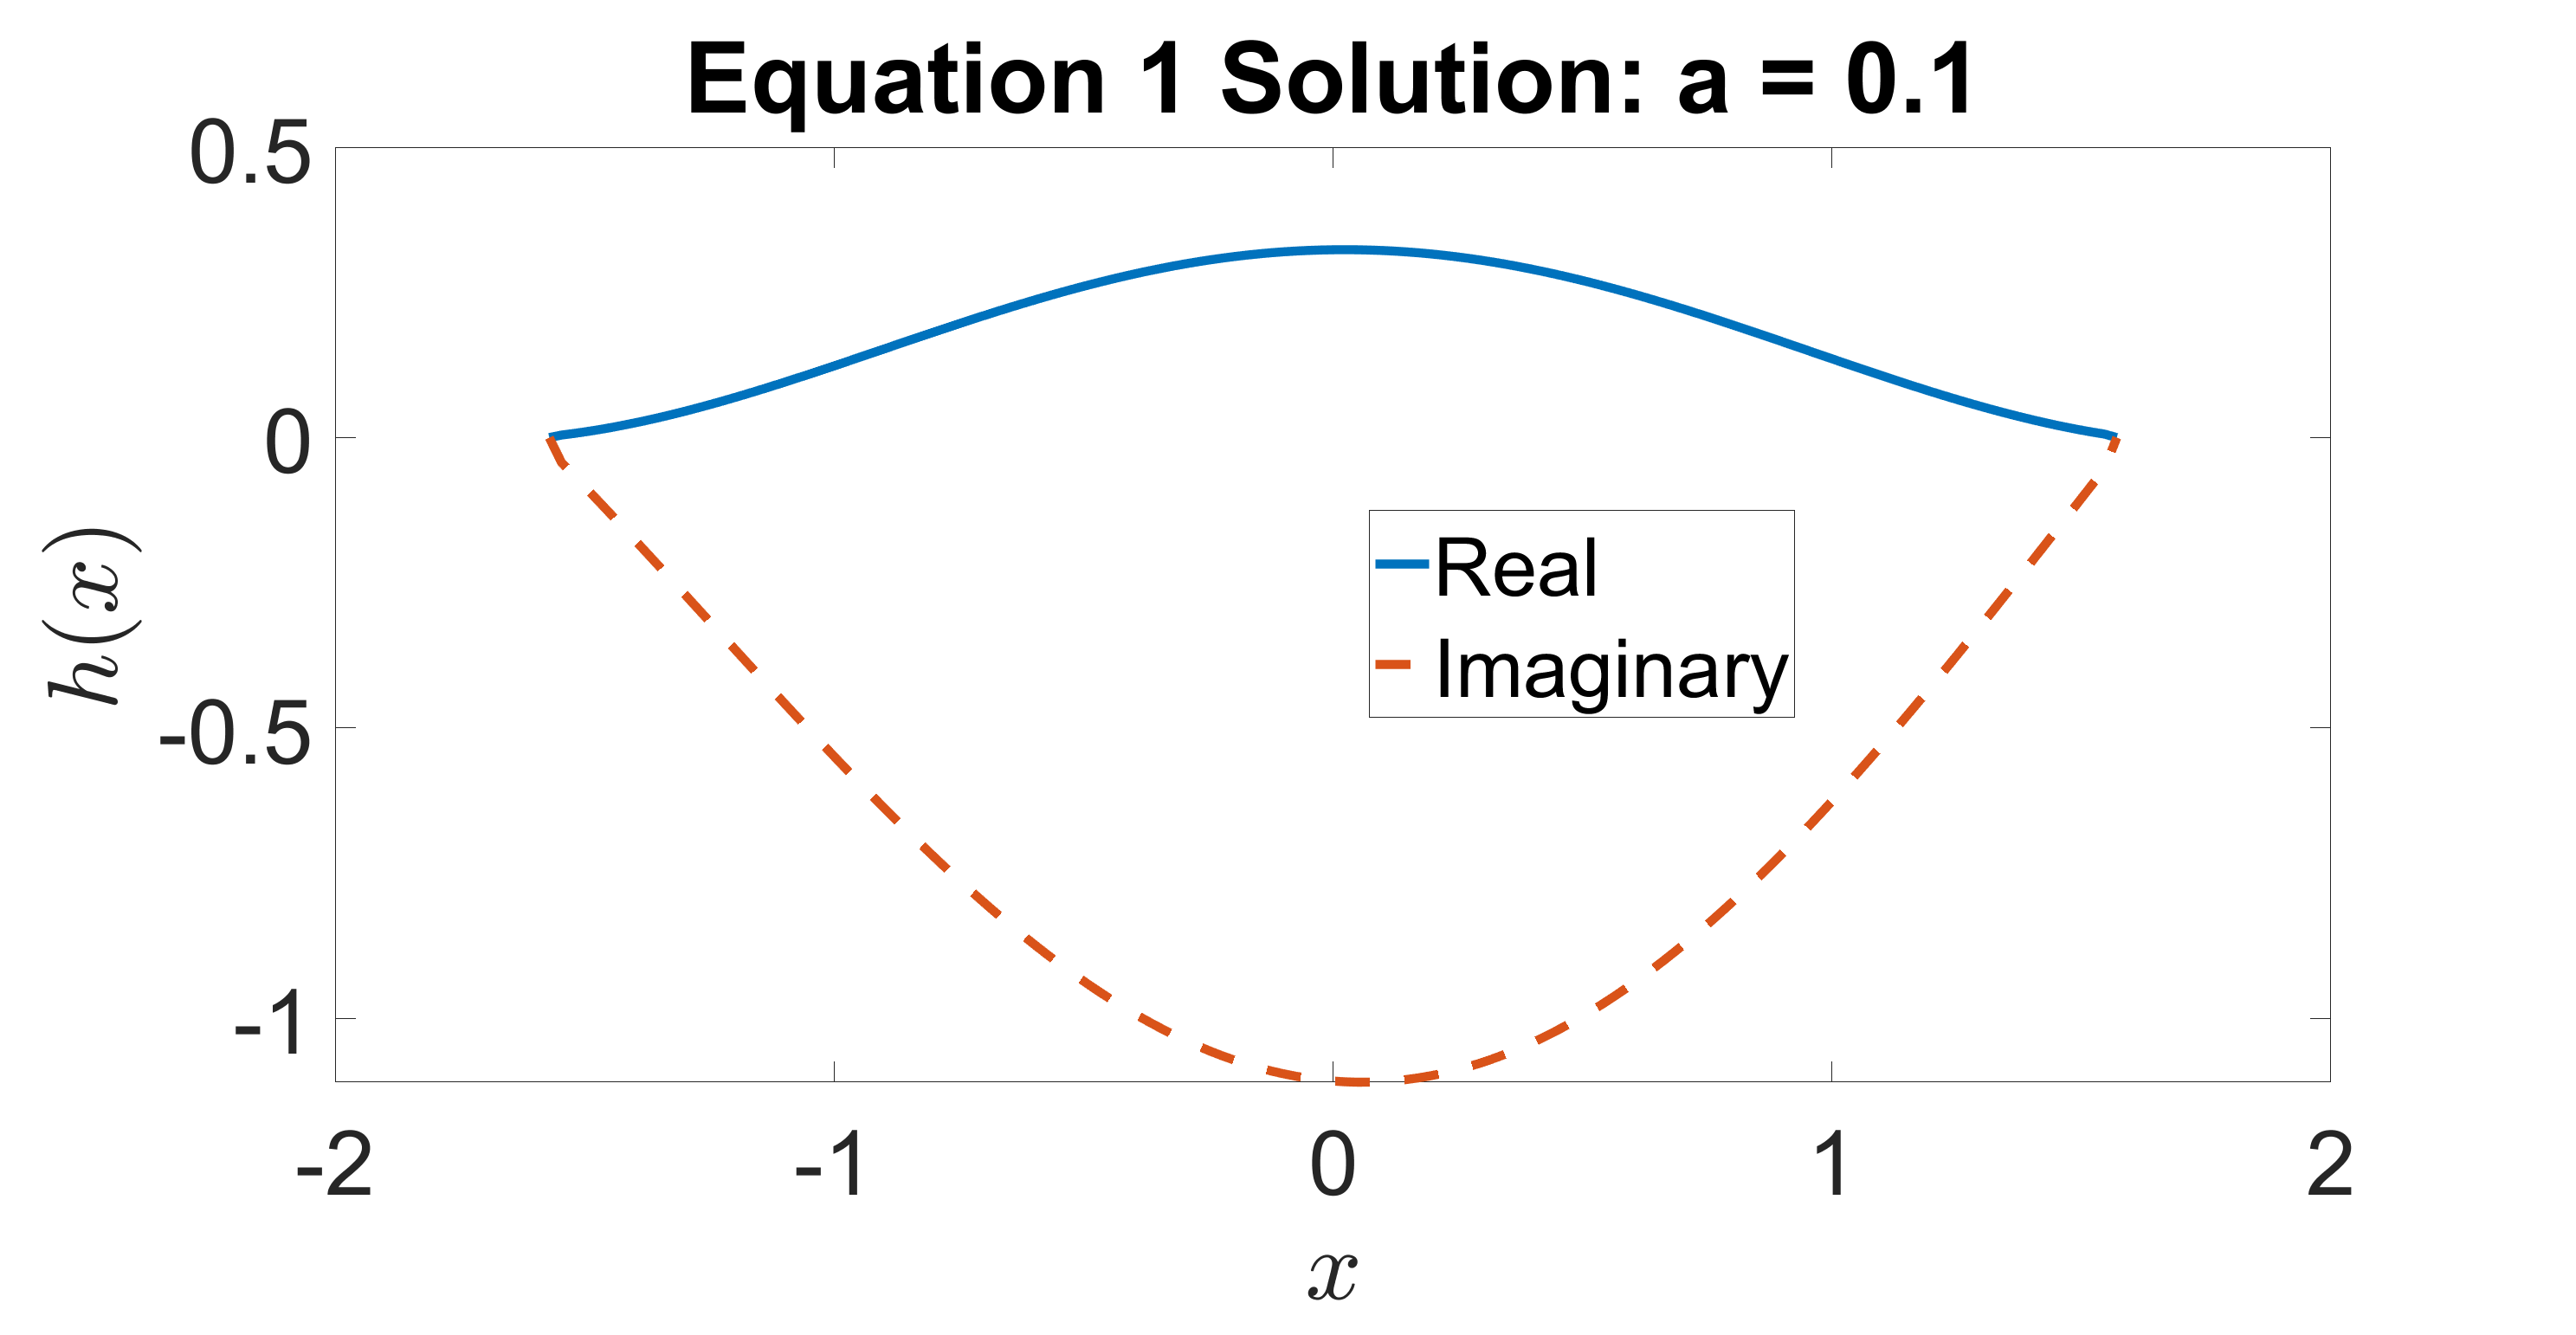
\includegraphics[width=5in]{ide21.png}}
    \vspace{0.3cm}
    \subfloat{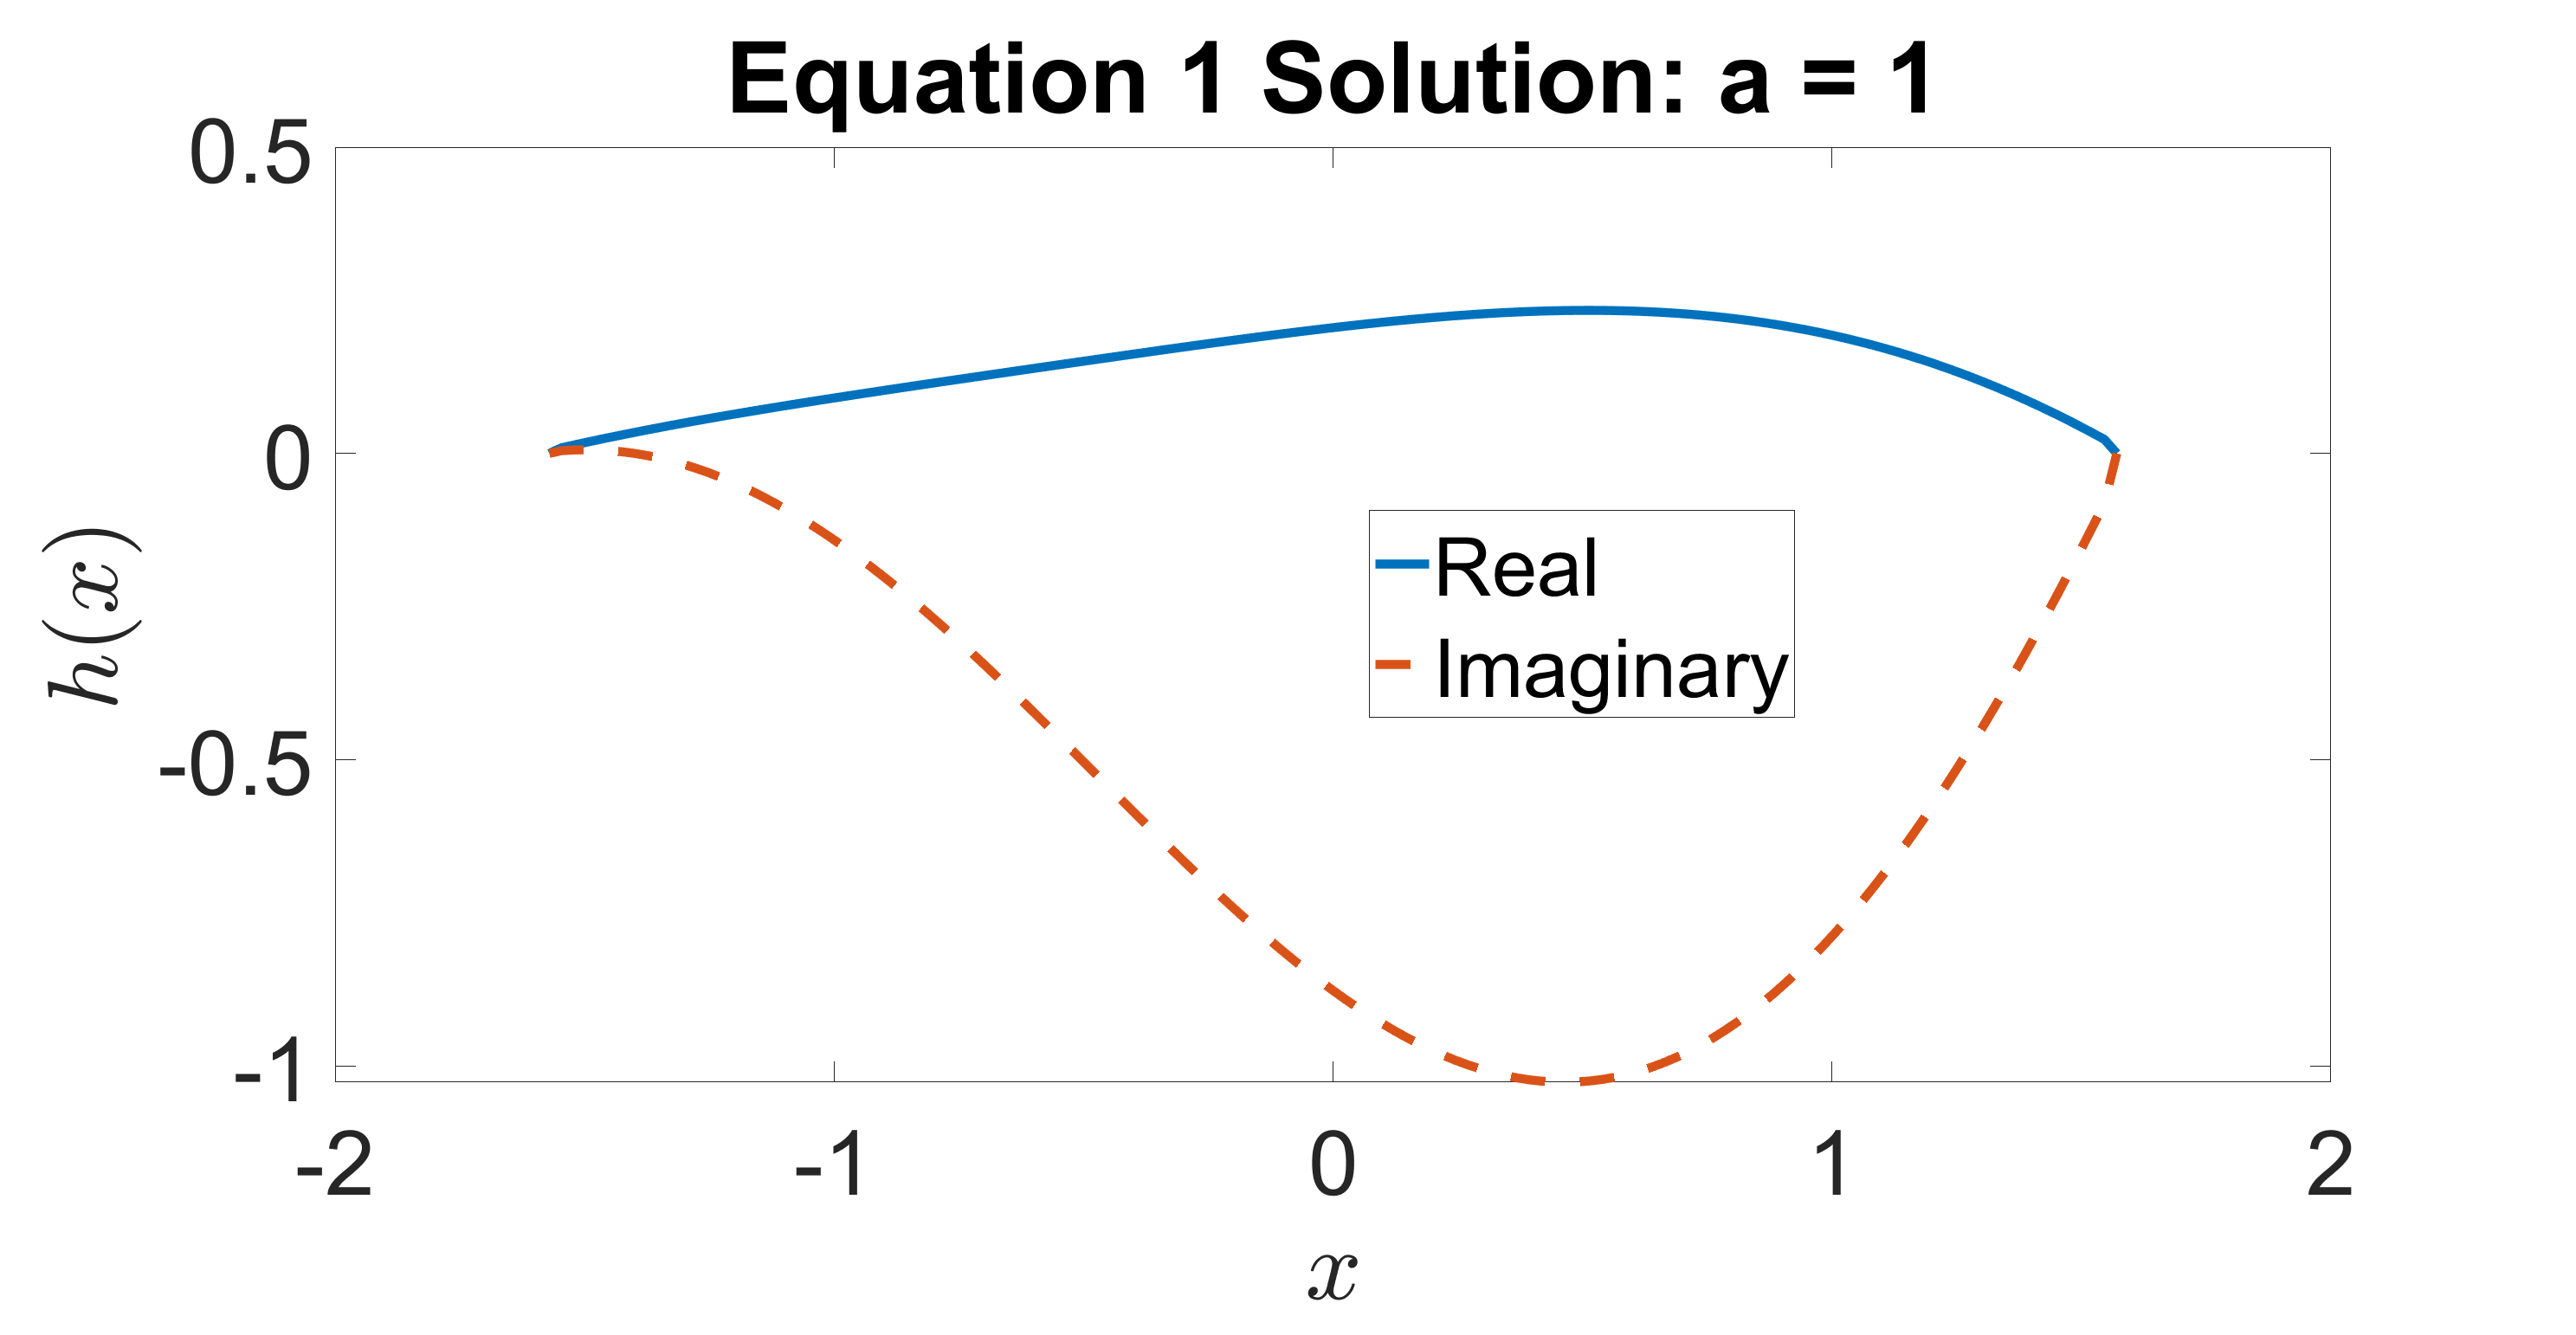
\includegraphics[width=5in]{ide2.png}}
    \caption{We give the complex solutions to equation 1 for $a = 0.1$ and $a = 1.0$. In both cases we specify a resolution of 128 grid points.}
    \label{solns1}
\end{figure}
\clearpage
We continue by attempting to describe the error with increasing resolution. Recall that as we double the resolution and compare the norm of the difference in solutions, we expect that value to decrease exponentially.
More specifically, the $log_2$ of the quotient of these norms is the order of convergence. 
If $h_{N}$ is the solution with resolution $N$ and $h_{N/2}$ is the solution with resolution $N/2$, then assuming we compare the appropriate values, we have that
\begin{align}
    OOC &\equiv \log_2 \frac{|h_{N} - h_{N/2}|_{\infty}}{|h_{2N} - h_{N}|_{\infty}}  
\end{align}
where $OOC$ refers to the order of convergence and we are taking an $L-\infty$ norm.
Plots of the ``error'' norms are given in Figure~\ref{fig:error}.

\begin{figure}[H]
    \centering
    \subfloat{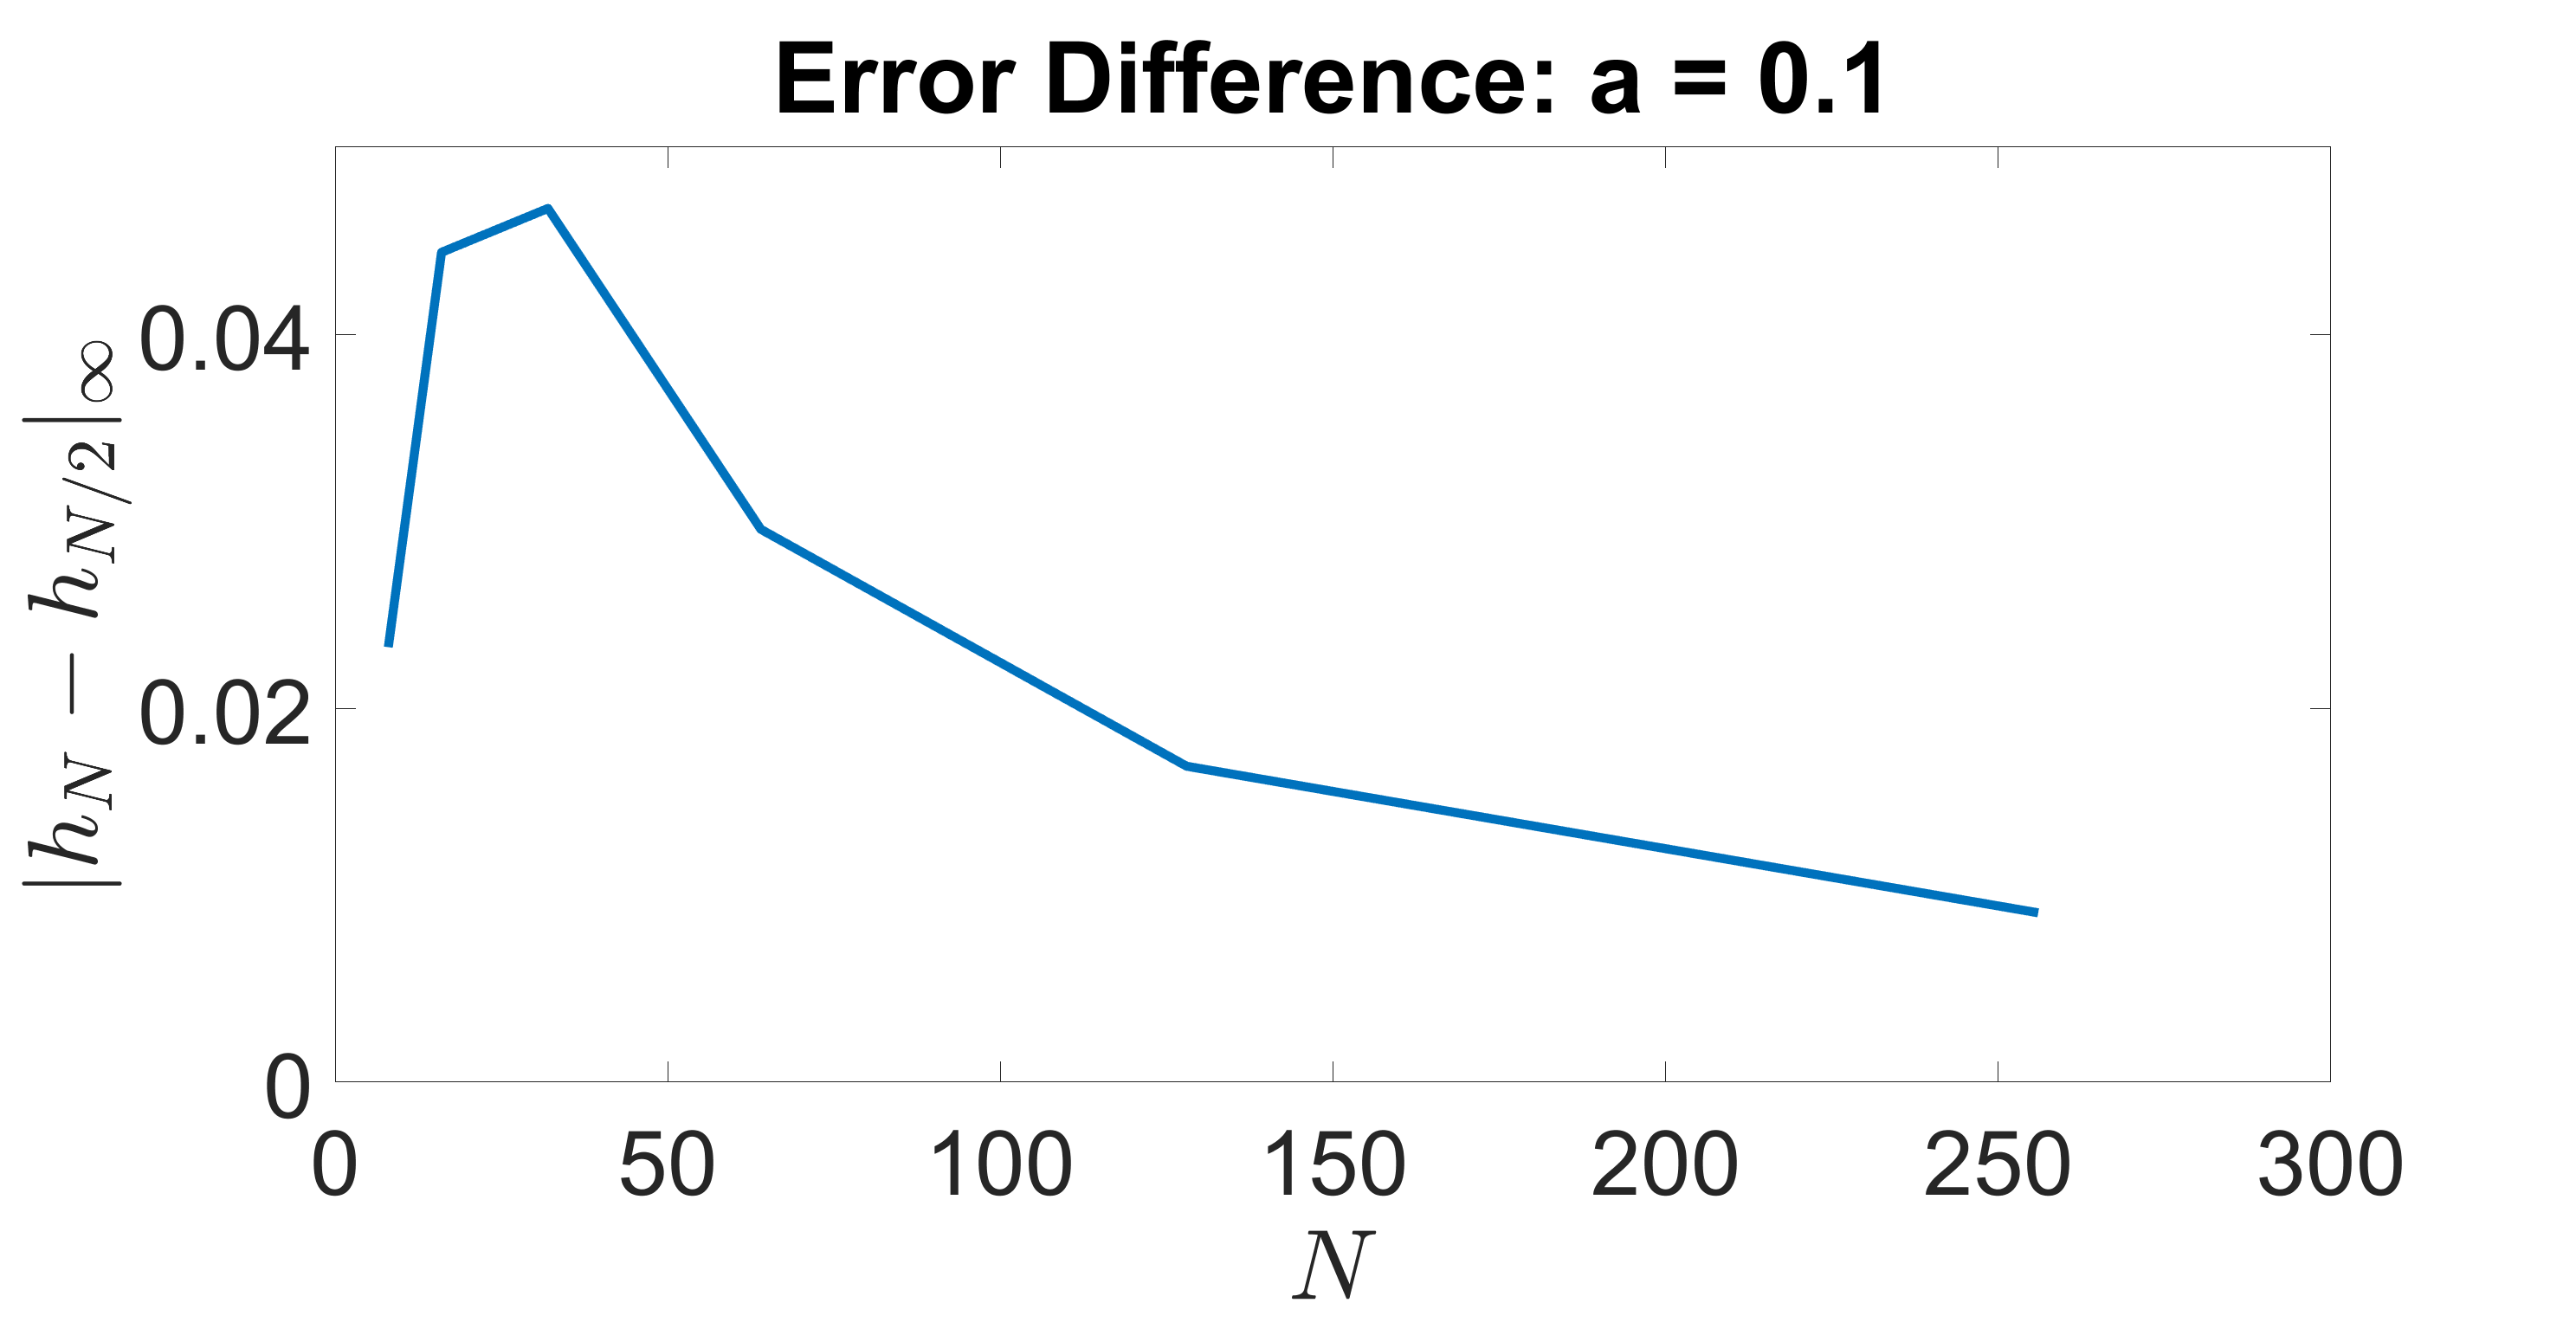
\includegraphics[width=5in]{errors1.png}}
    \vspace{0.3cm}
    \subfloat{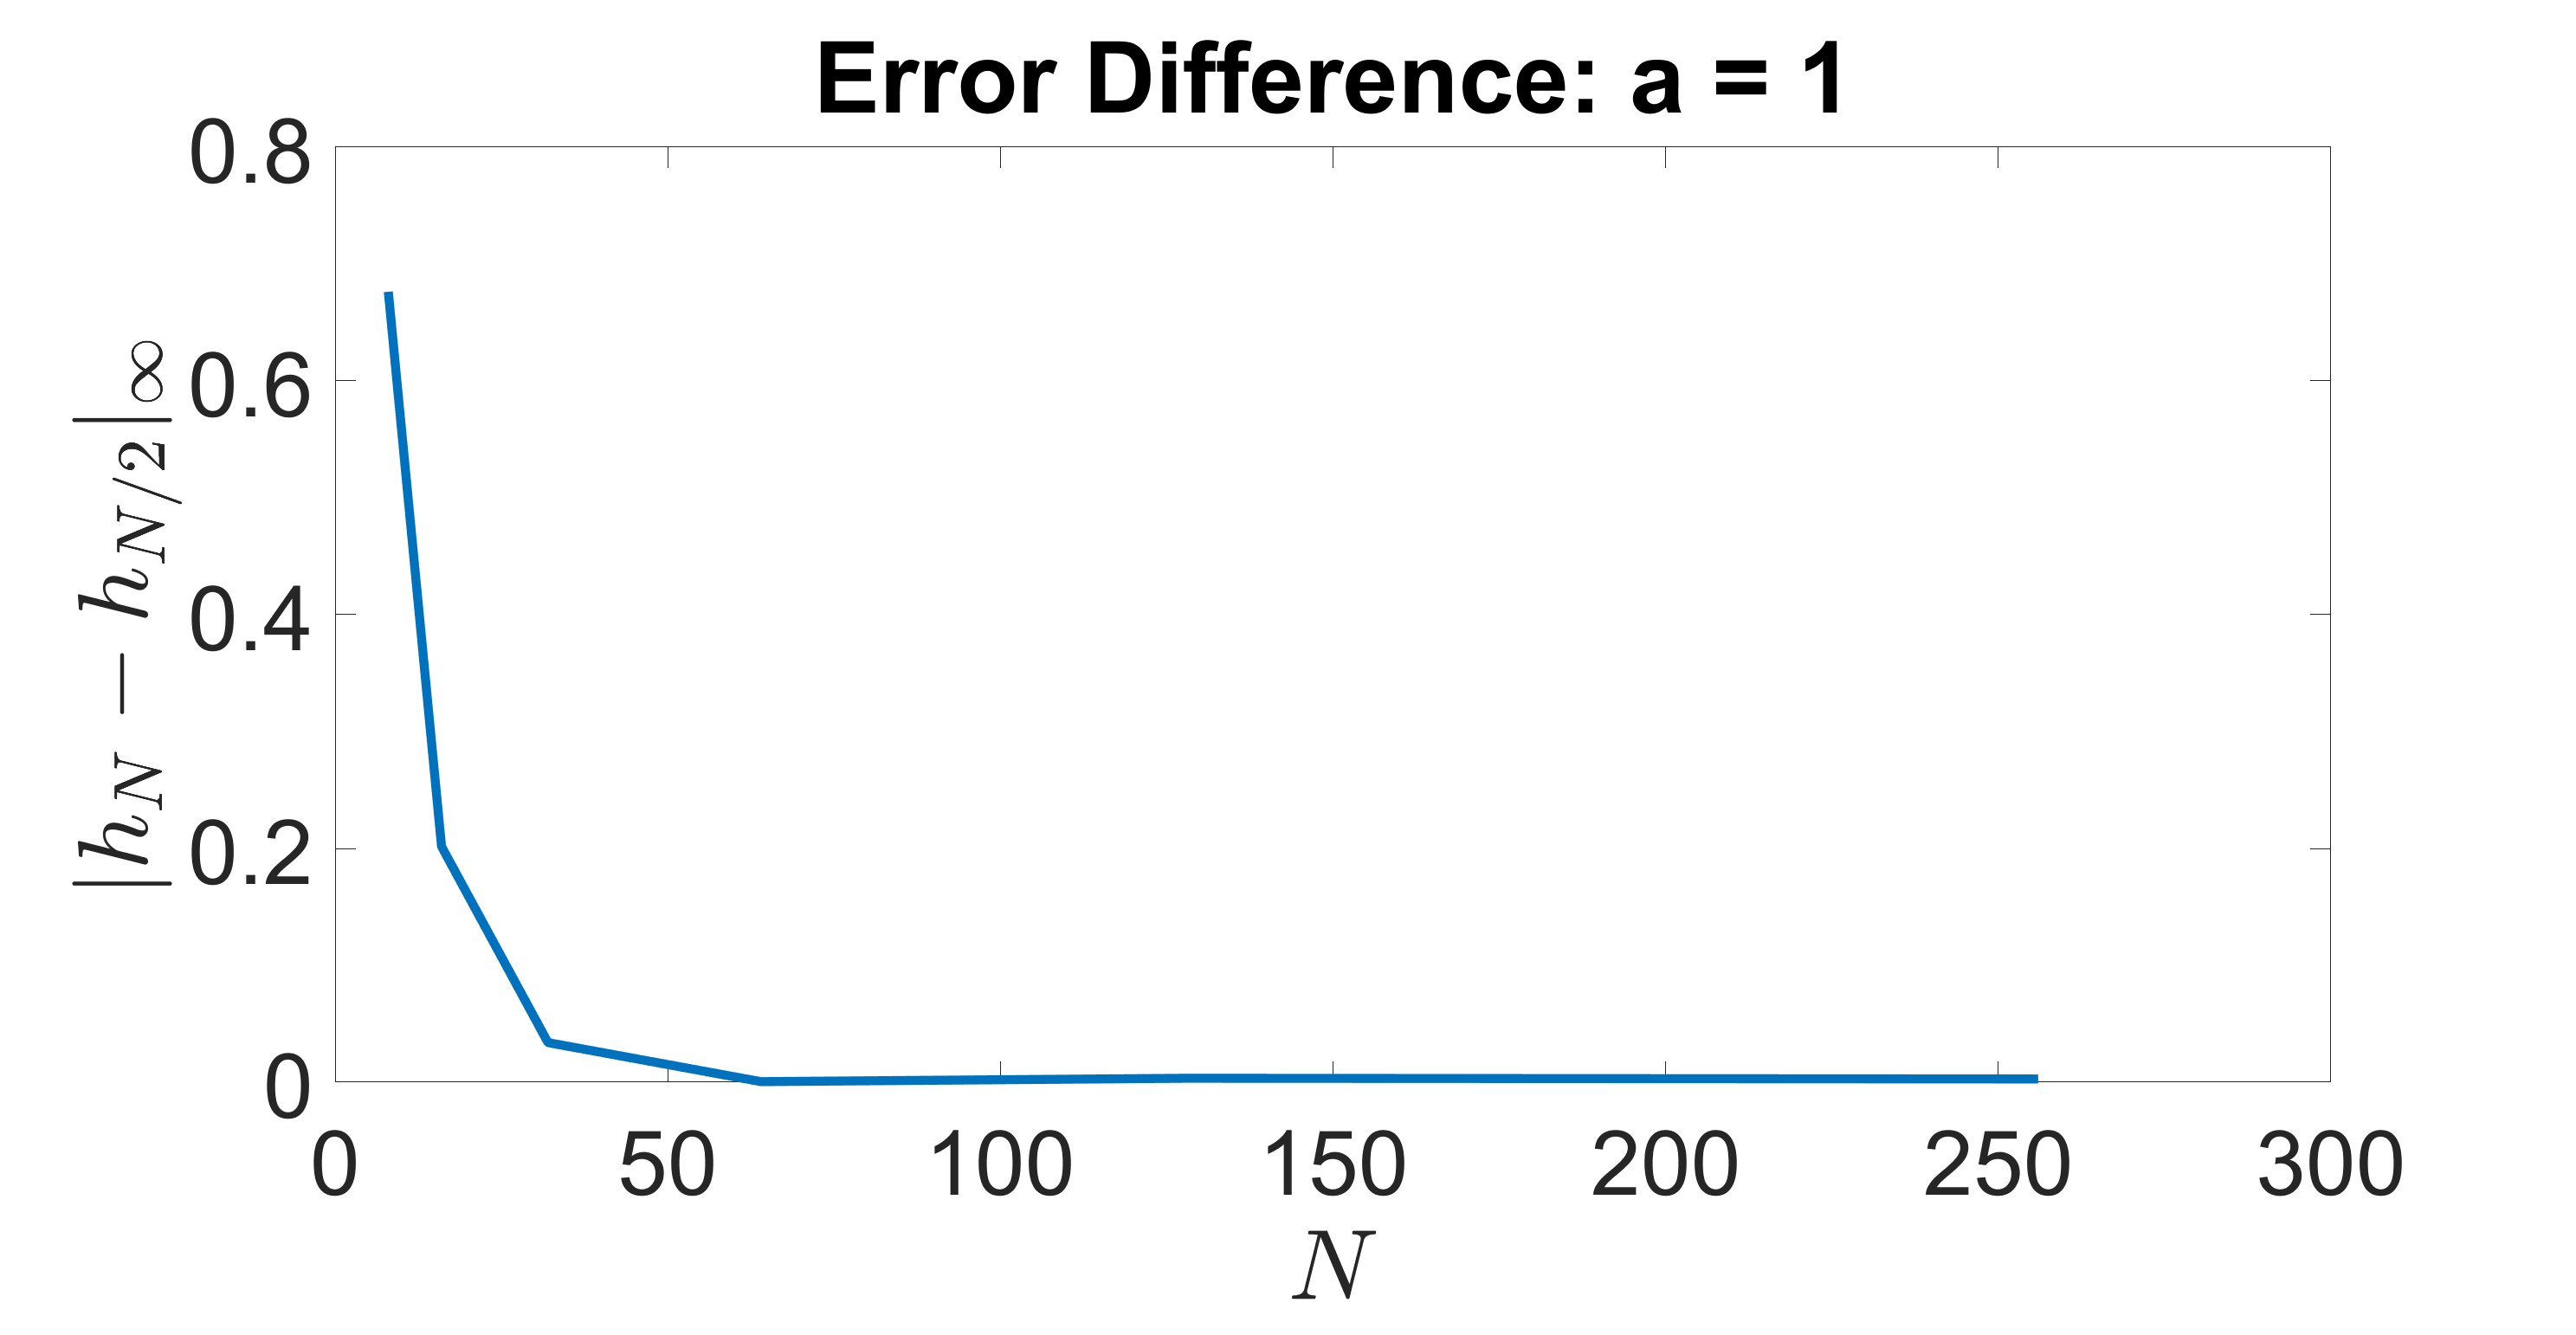
\includegraphics[width=5in]{errors2.png}}
    \caption{Here we give the ``error'' norms with increasing resolution. It is clear in both cases that once a sufficiently large resolution $N$ is employed, the norms appear to decrease exponentially, with different factors in each case.}
    \label{fig:error}
\end{figure}

\clearpage
\vfill
\vfill
Finally, we report the norms of the ``errors'' and their respective quotients over various resolutions $N$ in Figure~\ref{fig:tab}.
We observe different orders of convergence for various $a$.
In the case of $a = 0.1$, we fail to achieve second (or even first) order convergence, with $OOF \approx 0.9$.
Why we fell short of the intended goal is not clear.
In constrast, we find that for $a = 1$, the algorithm converges quite rapidly with increasing $N$.
Here we appear to achieve second order convergence.
It should be noted that with increasing $a$, we ought to investigate large resolutions due to the possible relationship between the spatial wavenumber $a$ and the small-scale structure of $h$.
\vfill

\begin{figure}[H]
    \centering
    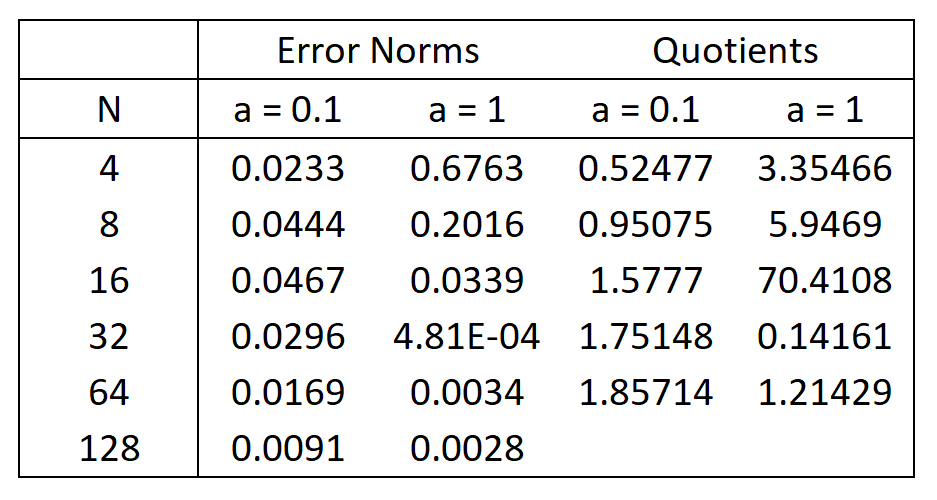
\includegraphics[width=3.5in]{errors_tab.PNG}
    \caption{Solution difference norms and their quotients for various resolutions and both values of $a$.}
    \label{fig:tab}
\end{figure}
\vfill
\section*{Discussion}
Recall (from your 445 class!) that high frequency can be solved more readily via relaxation methods.
We note that $a$ really controls the eigenfunctions of the homogeneous problem.
Larger $a$ values are associated with high frequency modes.
The solution reflects this as asymmetries and smaller-scale variation.
Further, we see rapid convergence with increased $a$, suggesting that possibly the \texttt{MATLAB} solver is optimized to use indirect (possibly relaxation-related) matrix solvers on larger problems.
Just speculating!

We failed to approximate the solution here with the same fidelity as in previous assignments.
Given more time this would something clearly worth investigating, though it could simply be due to \texttt{MATLAB}'s integration tools, that seems unlikely.
Generally in cases like this, it's the grad student's fault and not the massive software company's.
Though we used low order of convergence methods, we were able to solve this surprisingly complicated singular equation with great accuracy (I assume).
It's easy to see that these sorts of problems can become arbitrarily complicated, with the potential for higher spatial dimension, nonlinear deformation of the membrane, etc.
\vfill


\clearpage
\begin{thebibliography}{9}
    \bibitem{wolfram_hankle} Weisstein, Eric W. "Hankel Function of the First Kind." From MathWorld--A Wolfram Web Resource. \url{https://mathworld.wolfram.com/HankelFunctionoftheFirstKind.html}
    
    \bibitem{bessel1} Weisstein, Eric W. "Hankel Weisstein, Eric W. "Bessel Function of the First Kind." From MathWorld--A Wolfram Web Resource. 
    \url{https://mathworld.wolfram.com/BesselFunctionoftheFirstKind.html}

    \bibitem{bessel2} Lambers, Jim. "Bessel Functions of the Second Kind"
    \url{http://www.math.usm.edu/lambers/mat415/lecture16.pdf}

    \bibitem{bessel22} Viktorovitch, M. "A boundary element solution to the vibration problem of bidimensional structures on a wide frequency range"
    \url{https://www.witpress.com/Secure/elibrary/papers/BE95/BE95025FU.pdf}
\end{thebibliography}
\end{document}
